\chapter{Architecture technique}\label{Architecture_technique}

\section{Application}
L'IHM est réalisé en langage C++ à l'aide du framework Qt.
\begin{notation}
L'application doit être réalisée en client lourd.
Il a été exclu l'éventualité d'utiliser un serveur en local (sur les postes client) c'est pourquoi les langages comme PHP ont été exclus.
\\
En outre le choix a été fait de préférer un langage qui soit~:
\begin{enumerate}
	\item orienté objet (ce qui exclu les langages comme C)~;
	\item multiplateforme~;
	\item suffisamment vieux pour avoir été durement éprouvé (ce qui exclu les langages comme Ruby)~;
	\item facile à prendre en main (d'où le choix du framework Qt)~;
	\item performant et peu couteux en mémoire (ce qui exclu les langages comme Java)~;
	\item compatible avec les divers autres éléments utilisés (SGBDR, LDAP, XML, ...)~;
\end{enumerate}
\end{notation}

\section{Authentification}
L'authentification est gérée par un annuaire LDAP actuellement en cours d'étude et de développement.

\clearpage
\section{Données}\label{DonneesTechnique}

\newcommand{\Qt}{\href{http://qt-project.org/}{Qt}\xspace}

% Indications :
%  Stockage (coté client, coté serveur, SGBD, format, ...)
%  Transfert (format, norme, ...)
%  Import/Export...
% 
% Bon courage ;-)

\subsection{Problématique}
Ce chapitre traite du stockage et du formatage des données sur les différents postes, et dans les différentes situations d'utilisation précédemment décrites. \\
Cette problématique est divisée selon trois points clés~:
\begin{itemize}
	\item le stockage~;
	\item le transfert~;
	\item l'importation et l'exportation.
\end{itemize}

\subsection{Le stockage}
Cette section développe en détail les différents type de stockage au sein de l'architecture clients/serveurs.

\subsubsection{Côté serveur}
Le stockage des données côté serveur se fait grâce au SGDBR MySQL. Cette solution a été retenue pour plusieurs raisons~:
\begin{itemize}
	\item solution traitant rapidement les données~;
	\item solution compatible avec la plupart des systèmes d'exploitation (Windows, GNU/Linux, MacOS, ...)~;
	\item solution facile à utiliser~;
	\item solution pouvant facilement s'interfacer à l'aide d'API diverses~;
	\item solution de prédilection de notre entreprise, ce qui garantit une interopérabilité maximale.
\end{itemize}

\subsubsection{Côté client}
Le stockage des données côté client se fait soit via deux représentations d'une base de données locale : une tournant sur MySQL et un autre utilisant des fichiers au format XML. s'il est possible d'effectuer la synchronisation avec la base de donnée centrale et que le périphérique le permet, la première représentation est choisi par défaut. Si la synchronisation au serveur central est indisponible, le stockage des données est fait par la deuxième représentation de la base au format XML. \\
Le choix de l'utilisation des fichiers XML est dû aux raisons suivantes~:
\begin{itemize}
	\item format universel, compatible à l'import/export avec la plupart des SGDBR (dont MySQL)~;
	\item taux de compression assez important sur ce format, ce qui peut favoriser le transfert des données dans des situations où la connexion est limitée~;
	\item exploitable sur les périphériques Android.
\end{itemize}

\subsubsection{Structuration des données}
%% Mj %% Librairie MjMcd en cours de développement...
%\begin{figure}[htbp]
%	\centering
%	\begin{MjMcd}
%		\MjMcdEntity{Requisition}{
%			RequisitionCountryCode	: VARCHAR(3)	\\	%
%			RequisitionId			: VARCHAR(25)	\\	%
%			ForCostEstimate			: NUMERIC()		\\	%
%			ForPurchase				: NUMERIC()		\\	%
%			WhDispatchRelease		: NUMERIC()		\\	%
%			RequisitionDate			: DATE			\\	%
%			DesiredDeliveryDate		: DATE			\\	%
%			Project					: VARCHAR()		\\	%
%			Activity				: VARCHAR()		\\	%
%			MCode					: VARCHAR()		\\	%
%			TransportMeans			: TRANSPORTMEAN		%
%		}
%	\end{MjMcd}
%	\caption{Structuration des données dans le SGBDR~: le MCD}
%	\label{DonneesStructurationSgbdrMcd}
%\end{figure}
%\begin{figure}[htbp]
%	\centering
%	\caption{MCD (Modèle Conceptuel des Données)}
%	\label{DonneesStructurationSgbdrMcd}
%\end{figure}

\subsubsection{Génération de la base de données}
Le bon fonctionnement de la base de données s'appuie sur les fichiers suivants~:
\begin{enumerate}
	\item \emph{Database.properties}~;
	\item \emph{Database.mcd}~;
	\item \emph{Database.sql}.
\end{enumerate}

\paragraph{Database.properties}
Ce fichier définit les propriétés indispensables à la connexion avec la base de données.
Il se présente sous la forme suivante~:
\lstinputlisting[language=Bash]{Database.properties}
\label{Database.properties}
\begin{enumerate}
	\item \emph{dbDriver} est le driver Qt correspondant à la base de données considérée (dans le cas présent MySQL)~;
	\item \emph{dbHostName} est l'adresse URL de la base de données (ici localhost)~;
	\item \emph{dbUserName} est le nom d'utilisateur (ici root)~;
	\item \emph{dbPassword} est le mot de passe d'utilisateur (ici aucun)~;
	\item \emph{dbName} est le nom que l'on souhaite donner à la base de donnée considérée (ici GkLogistic). Ce dernier est optionnel, et ne présente de réel intérêt que dans le cas où plusieurs bases de données distinctes seraient utilisées.
\end{enumerate}
Via \Qt, l'utilisation de ces informations de connexion se fait, par exemple, de la façon suivante~:
\lstinputlisting[language=Qt]{Database.example.cpp}
\label{Database.example.cpp}

\paragraph{Database.mcd}
Ce fichier définit le MCD (Modèle Conceptuel des Données) éditable par l'intermédiaire de l'outil de développement \JMerise.
Ce dernier permet, entre autres choses, de générer le fichier de script \emph{Database.sql}.

\paragraph{Database.sql}
Ce fichier définit l'architecture relationnelle (en SQL) de la base de données.
Ce script est exécuté quand la base de données n'existe pas, et la crée.

\paragraph{Database.xml}
Ce fichier définit l'architecture relationnelle (en XML) de la base de données.
Ce script est exécuté quand la base de données n'existe pas, et la crée.

\subsection{Le transfert}
Le transfert des données quant à lui, est réalisé selon un format et une norme qui est préalablement défini.

\subsubsection{Format}
Eu égard des solutions retenues pour le transfert des données, le transfert des données se fera grâce à des fichiers XML. \\
La possibilité est donnée de compresser ces fichiers, dans un premier temps au format \emph{ZIP}, mais ce choix peut être remis en question selon les observations réalisées sur les données de test, afin de retenir une éventuelle meilleure solution.

\subsubsection{norme}
% Définir la norme du format XML correspondant à une table SQL
% avec une DTD associée.
% 
% Exemple de DTD pour une personne :
% 
% <!ELEMENT personne (nom,prenom,telephone),email? >
% <!ELEMENT nom (#PCDATA) >
% <!ELEMENT prenom (#PCDATA) >
% <!ELEMENT telephone (#PCDATA) >
% <!ELEMENT email (#PCDATA) >

\subsection{L'import/export de données}
L'import et l'export de données se fait directement via une fonctionnalité de l'outil côté client, qui permet de sélectionner les données à importer dans le contexte spécifique, ainsi que les données à exporter vers le serveur central, toujours selon ce contexte.
Comme décrit dans la partie traitant de ce sujet, l'import/export de données est réalisé selon différents supports (réseau, support physique) à la discrétion de l'exploitant.


\clearpage
\section{Sauvegarde}\label{SauvegardeTechnique}
\label{Architecture_technique_de_sauvegarde}

\subsection{Problématique}
La suite logicielle permet de synchroniser des données, à la fois entre postes clients et serveur local, mais également entre serveur local et serveur central, et ce, via les différentes architectures ci dessous.

\subsection{Cluster}
Une première solution utilisant la technologie du \emph{cluster} peut être envisagée.
Cette technique permet de créer un groupe logique de serveurs qui s'exécutent simultanément tout en donnant l'impression aux utilisateurs de ne constituer qu'un seul serveur.
En considérant le matériel existant, et le fait que l'achat de serveur dédié pour ce cluster serait coûteux au client, une solution de \emph{clustering} peut être effectuée grâce à de simples postes clients qu'il faut configurer comme des serveurs.
Dans l'architecture proposée (voir figure \ref{SchemaCluster}), deux postes clients (configurés comme des serveurs maître/esclave) sont reliés directement par un câble ethernet, ce qui permet de dupliquer au fur et à mesure toutes les données.
Le serveur maître transmet les données au serveur esclave, et en cas d'incident sur le serveur maître, c'est le serveur esclave (ou de secours) qui reprend la main.

\begin{figure}[htbp]
	\centering
	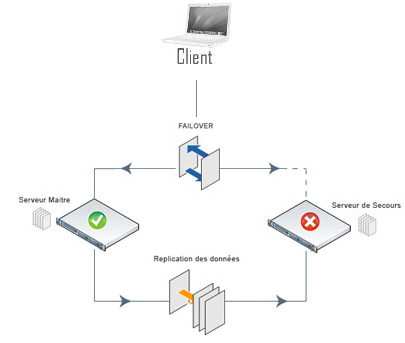
\includegraphics[scale=0.9]{Images/SchemaCluster.png}
	\caption{Cluster, serveur maître et esclave directement connectés}
	\label{SchemaCluster}
\end{figure}

%\begin{figure}[htbp]
%	\centering
%	\begin{tikzpicture}
%	    % Styles :
%		\tikzstyle{titre}=[rectangle,draw,fill=white,text=black]
%		\tikzstyle{symbole}=[rectangle,text=black, scale=4]
%		\tikzstyle{serveurloc1}=[rectangle,draw,fill=blue!50,text=white, minimum height=2cm]
%		\tikzstyle{serveurloc2}=[rectangle,draw,fill=yellow!50,text=black, minimum height=2cm]
%		\tikzstyle{serveurcentral}=[rectangle,draw,fill=violet!50,text=black, minimum height=2cm]
%		
%		% #### CADRE VERT :
%		% Fond :
%		\draw[fill=green!10] (0,6) rectangle (16, 11);
%		\draw[fill=red!10] (2,11) rectangle (11, 6);
%		% Titres :
%		\node[titre] at (6.50,7.00) {Serveur local};
%		% Serveurs :
%		\node[serveurloc1] at (4.00,8.50) {Serveur maître};
%		\node[serveurloc2] at (9.00,8.50) {Serveur esclave};
%		\node[serveurcentral] at (14.00,8.50) {Serveur central};
%		% Traits :
%		\draw[line width=2pt] (1.5, 8.5) -- (2, 8.5);
%		\draw[line width=2pt] (5.5, 8.5) -- (7.5, 8.5);
%		\draw[line width=2pt] (11, 8.5) -- (12.5, 8.5);
%		% Utilisateurs :
%		\umlactor[x=1.00, y=8.50]{Utilisateur}
%	\end{tikzpicture}
%
%\caption{Cluster, serveur maître et esclave directement connectés}
%	\label{explicationcodeco}
%\end{figure}

Le serveur de secours est en \emph{hot standby}, c'est-à-dire qu'il reste allumé en mode passif, attendant que des requêtes clients soient reçues (requêtes qui sont envoyées au maître tant que ce dernier est actif).

\paragraph{Fail-over}
Dans le cadre d'une architecture serveur haute disponibilité, le \emph{fail-over} permet une reprise automatique inférieure à une minute sur le serveur de secours en cas de défaillance du serveur maître. Le \emph{fail-over} est donc la capacité d'un équipement à basculer automatiquement vers un chemin réseau redondant ou en veille.
Cette solution est préconisée sur les serveurs ou les architectures serveurs qui nécessitent une disponibilité permanente et un haut niveau de connectivité.
\\
Il existe deux utilisations du protocole \emph{fail-over}~:
\begin{itemize}
	\item mode statique~: chaque client est configuré pour basculer sur une URI précise si la standard ne répond plus~;
	\item mode dynamique~: le maître fournit dynamiquement l'URI de l'esclave aux clients qui peuvent la mettre à jour.
\end{itemize}
Le mode retenu est le mode statique, où chaque client a sa configuration et la conserve, aucune configuration spécifique n'est donc nécessaire pour le maître, et il faut simplement configurer sur l'esclave la connection avec le maître.

\paragraph{Réplication des bases de données en temps réel}
Les écritures sur le serveur maître sont répliquées en temps réel sur le serveur de secours, ne ralentissent pas le serveur maître et permettent de minimiser les pertes de données.
La réplication se fait par recopie des journaux de transactions entre le maître et l'esclave.
\\
Le mode de synchronisation choisi est le mode synchrone~: une transaction émise par un client n'est validée que si l'écriture sur le maître ainsi que la synchronisation avec le serveur de secours sont validées.
Ceci permet de s'assurer de la bonne duplication des données sur les deux serveurs. 

\paragraph{Limitations}
Seul un esclave à la fois peut être connecté au maître.
Un maître hors ligne ne peut être réintroduit qu'à froid.
Répliquer les données de l'esclave vers le maître une fois ce dernier remonté n'est pas automatique, cela nécessite une intervention manuelle.

\paragraph{Logiciel}
Apache Active MQ est un agent de messages open source, écrit en Java et associé avec un client Java Message Service.
Cette suite prend en charge divers protocoles de transport et précisément le protocole de fail-over qui permet de configurer les clients afin qu'ils basculent sur le serveur esclave en cas de non réponse du maître. 
Il permet aussi de charger les différentes configurations (clients, maître et esclave) conservées dans des fichiers XML. 

\subsection{Sauvegarde en dur}
Une deuxième solution peut être mise en œuvre de manière complémentaire au \emph{cluster} afin de mieux respecter la contrainte concernant l'intégrité des données.
Un support mobile de stockage est utilisé afin de directement sauvegarder le contenu des serveurs.
Le support peut être un disque dur, une clé USB, une carte mémoire...
Cette sauvegarde devra être effectuée toutes les six heures afin de permettre de remonter les données en cas de panne des deux serveurs.  


\clearpage
% ==============================================================================
\section{Synchronisation}

\label{SynchronisationTechnique}

% À charge à Bien Aimé et Ravi de remplir cette partie
% Indications :
%  Configuration des priorités etc.
%  Mode connecté (lié au serveur local)
%  Mode non connecté (à la Git-attitude)...
% 
% Bon courage ;-)

% ------------------------------------------------------------------------------
\subsection{Introduction}
L'objectif de cette section est de décrire les méthodes proposées afin de répondre au problème de synchronisation. Les échanges de données pouvant être limités (pas de réseau, liaison satellitaire uniquement) il convient de pouvoir choisir précisément les éléments que l'on souhaite synchroniser\footnote{Il est à noter que la synchronisation est bi-directionnelle : on reçoit les informations du serveur autant qu'on en envoie.}.\\
Pour permettre la gestion de ces éléments, on introduit la notion de \emph{priorité}; à chaque catégorie d'éléments (e.g. planning des transports, liste des fournisseurs, informations sur les véhicules, ...) peut être associée une priorité de laquelle dépendra la synchronisation ou non. À partir de cette \og{}hiérarchie d'importance\fg{}, on associe des \emph{profils de synchronisation} paramétrables qui - une fois activés - gère la synchronisation de façon transparente en fonction des choix de l'utilisateur.\\
Pour résoudre les problèmes de connexion et assurer le fonctionnement de la suite logicielle indépendamment de la liaison réseau, deux modes sont prévus :
\begin{itemize}
    \item Connecté
    \item Hors-ligne
\end{itemize}
L'utilisation de ces deux modes est décrit dans la Fig. \ref{explicationcodeco} : on utilise le mode connecté lorsque la liaison réseau est établie avec le serveur local; et le mode hors-ligne quand il n'y a pas de liaison avec le serveur local. Dans les deux cas, nous faisons abstraction de la liaison entre le serveur local et le serveur central dans la mesure où l'utilisateur ne se synchronisera qu'avec le serveur local.
% Schéma pour montrer la différence d'utilisation entre le mode connecté et hors ligne :
\begin{figure}[htbp]
    \centering
	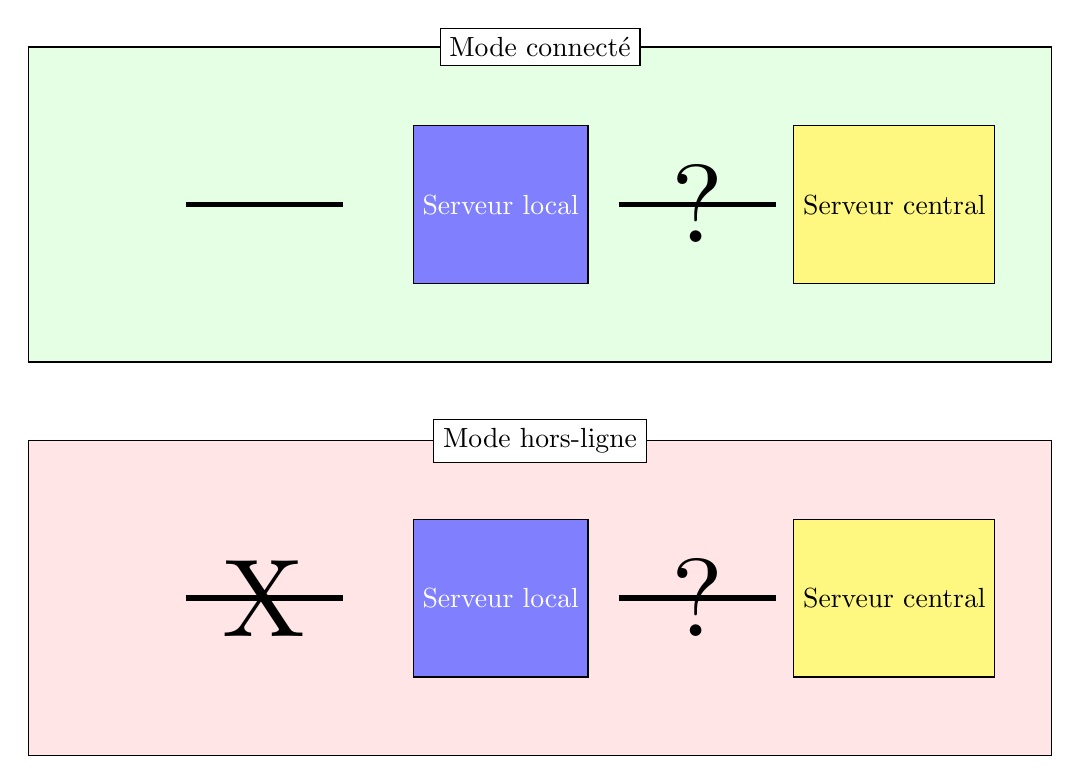
\begin{tikzpicture}
	    % Styles :
		\tikzstyle{titre}=[rectangle,draw,fill=white,text=black]
		\tikzstyle{symbole}=[rectangle,text=black, scale=4]
		\tikzstyle{serveurloc}=[rectangle,draw,fill=blue!50,text=white, minimum height=2cm]
		\tikzstyle{serveurcen}=[rectangle,draw,fill=yellow!50,text=black, minimum height=2cm]
	    % #### CADRE ROUGE :
		% Fond :
		\draw[fill=red!10] (0,0) rectangle (13, 4);
		% Titres :
		\node[titre] at (6.50,4.00) {Mode hors-ligne};
		% Serveurs :
		\node[serveurloc] at (6.00,2) {Serveur local};
		\node[serveurcen] at (11.00,2) {Serveur central};
		\node[symbole] at (8.50,2) {?};
		\node[symbole] at (3.00,2) {X};
		% Traits :
		\draw[line width=2pt] (2, 2) -- (4, 2);
		\draw[line width=2pt] (7.5, 2) -- (9.5, 2);
		% Utilisateurs :
		\umlactor[x=1.00, y=2]{Utilisateur}
		% #### CADRE VERT :
		% Fond :
		\draw[fill=green!10] (0,5) rectangle (13, 9);
		% Titres :
		\node[titre] at (6.50,9.00) {Mode connecté};
		% Serveurs :
		\node[serveurloc] at (6.00,7) {Serveur local};
		\node[serveurcen] at (11.00,7) {Serveur central};
		\node[symbole] at (8.50, 7) {?};
		% Traits :
		\draw[line width=2pt] (2, 7) -- (4, 7);
		\draw[line width=2pt] (7.5, 7) -- (9.5, 7);
		% Utilisateurs :
		\umlactor[x=1.00, y=7]{Utilisateur}
	\end{tikzpicture}
	\caption{Utilisation des modes connecté et hors-ligne}
	\label{explicationcodeco}
\end{figure}
    % TODO Schéma mode connecté
    % TODO Schéma mode hors-ligne
% Fin de la sous-section [Introduction]
% ------------------------------------------------------------------------------

% ------------------------------------------------------------------------------
\subsection{Gestion des priorités \& des profils de synchronisation}
Une priorité permettra à l'application de \og{}choisir\fg{} ce qui transitera sur le réseau. Cinq priorités seront définies (par ordre d'importance croissant) pour qualifier des éléments synchronisables :
\begin{enumerate}
    \item Négligeable
    \item Secondaire
    \item Normal
    \item Important
    \item Crucial
\end{enumerate}
L'utilisateur pourra gérer les priorités à synchroniser en les associant à un profil : lorsque l'utilisateur choisit un profil de synchronisation, seuls les éléments ayant une priorité inclue dans le profil sont synchronisés.
% Diagramme des CU pour la gestion des profils et des priorités :
\begin{figure}[htbp]
    \centering
	\begin{tikzpicture}
		\begin{umlsystem}[x=8.00,y=5.00,fill=yellow!10]{Priorités des éléments synchronisables}
			\umlusecase[x=0.00,y=1.00,name=MPrio]{Modifier la priorité d'un élément}
		\end{umlsystem}
		\begin{umlsystem}[x=8.00,y=0.00,fill=blue!10]{Profils de synchronisation}
			\umlusecase[x=0.00,y=0.00,name=ChProf]{Choisir un profil}
			\umlusecase[x=0.00,y=1.00,name=EProf]{Éditer un profil}
			\umlusecase[x=0.00,y=2.00,name=CrProf]{Creer un profil}
			\umlusecase[x=0.00,y=3.00,name=SProf]{Supprimer un profil}
		\end{umlsystem}
		\umlactor[x=0.00,y=3.00]{Utilisateur}
		\umlassoc{Utilisateur}{MPrio}
		\umlassoc{Utilisateur}{ChProf}
		\umlassoc{Utilisateur}{EProf}
		\umlassoc{Utilisateur}{CrProf}
		\umlassoc{Utilisateur}{SProf}
	\end{tikzpicture}
	\caption{Diagramme des cas d'utilisation pour la synchronisation}
	\label{ucsynchro}
\end{figure}
% Fin de la sous-section [Gestion des priorités]
% ------------------------------------------------------------------------------

% ------------------------------------------------------------------------------
\subsection{Mode connecté}
Dans ce mode, on suppose qu'il y a une liaison réseau entre l'utilisateur et le serveur local; toutes les modifications sont effectuées en \og{}temps réel\footnote{Un écart de temps pourra être constaté dans le cas où le réseau n'offre qu'un faible débit.}\fg{}. Pour ce mode, l'utilisateur doit :
\begin{enumerate}
    \item Se connecter
    \item Utiliser la suite logicielle
    \item Se déconnecter après utilisation
\end{enumerate}
L'utilisateur ne pourra effectuer que les modifications dont il a les \emph{permissions}.
% Diagramme des CU pour le mode connecté :
\begin{figure}[htbp]
    \centering
	\begin{tikzpicture}
		\begin{umlsystem}[x=5.00,y=0.00,fill=green!10]{Mode connecté}
			\umlusecase[x=1.00,y=1.50,name=Co]{Se connecter}
			\umlusecase[x=0.00,y=3.00,name=Modif, width=2cm]{Effectuer des modifications}
			\umlusecase[x=6.00,y=1.50,name=ChMode, width=2cm]{Choisir le mode connecté}
			\umlusecase[x=0.00,y=0.00,name=Deco]{Se déconnecter}
		\end{umlsystem}
		\umlactor[x=1.00,y=1.00]{Utilisateur}
		\umlinclude{Co}{ChMode}
		\umlinclude{Deco}{Co} 
		\umlinclude{Modif}{Co} 
		\umlassoc{Utilisateur}{Co}
		\umlassoc{Utilisateur}{Modif}
		\umlassoc{Utilisateur}{Deco}
	\end{tikzpicture}
	\caption{Diagramme des cas d'utilisation pour le mode connecté}
	\label{ucmodeco}
\end{figure}
% Fin de la sous-section [Mode connecté]
% ------------------------------------------------------------------------------

% ------------------------------------------------------------------------------
\subsection{Mode hors-ligne}
Contrairement au mode conecté, le mode hors ligne permet à l'utilisateur de modifier toutes les informations dont il dospose localement. Lorsqu'il souhaitera synchroniser ses informations avec le serveur, il devra se connecter et c'est à ce moment là que le serveur vérifiera que l'utilisateur n'outrepasse pas les droits qui lui sont accordés. Si c'est le cas, le serveur rejettera les modifications locales.
% Diagramme des CU pour le mode hors ligne :
\begin{figure}[htbp]
    \centering
	\begin{tikzpicture}
		\begin{umlsystem}[x=5.00,y=0.00,fill=red!10]{Mode hors-ligne}
			\umlusecase[x=4.50,y=0.20,name=Co]{Se connecter}
			\umlusecase[x=0.00,y=3.00,name=Modif, width=2cm]{Effectuer des modifications}
			\umlusecase[x=6.00,y=3.00,name=ChMode, width=2cm]{Choisir le mode hors-ligne}
			\umlusecase[x=0.00,y=1.00,name=Sync, width=2cm]{Synchroniser avec le serveur}
		\end{umlsystem}
		\umlactor[x=1.00,y=1.00]{Utilisateur}
		\umlinclude{Co}{ChMode}
		\umlinclude{Sync}{Co} 
		\umlassoc{Utilisateur}{Modif}
		\umlassoc{Utilisateur}{Sync}
	\end{tikzpicture}
	\caption{Diagramme des cas d'utilisation pour le mode hors-ligne}
	\label{ucmodedeco}
\end{figure}
% Fin de la sous-section [Mode hors-ligne]
% ------------------------------------------------------------------------------

% ------------------------------------------------------------------------------
\subsection{Gestion des conflits}
Durant la synchronisation, que ce soit en mode connecté ou hors-ligne, des conflits peuvent survenir au niveau du contenu des informations. Dans ce cas, l'utilisateur est averti du conflit et des informations qu'il touche et il lui revient le soin de les gérer en choisissant explicitement ce qui est correct et qui doit être enregistré sur le serveur.\\
Afin de savoir si la version des informations sur le serveur est plus récente (ou plus vieille) que la version locale, un horodatage est mis en place tel que :
\begin{itemize}
    \item Chaque modification locale est horodatée avec l'heure locale
    \item À la synchronisation, l'écart temporel entre l'heure locale et l'heure serveur est mesuré\footnote{Par exemple, supposons que la machine locale retarde de deux heures : si une information a été modifiée à 17h (heure serveur) et qu'une modification est apportée à 16h le même jour en local, l'écart de deux heures entre les deux machines est mesuré lors de la synchronisation (i.e. deux heures) et permet de dater réellement la modification en local et ainsi déterminer laquelle succède à l'autre. À cette fin, l'application enregistre les éventuels changements d'heure oppérés en local pour notifier le serveur des écarts d'horodatage.}
\end{itemize}
% Fin de la sous-section [Gestin des conflits]
% ------------------------------------------------------------------------------

% Fin de la section [Synchronisation]
% ==============================================================================


\clearpage
